\documentclass[xcolor=dvipsnames,aspectratio=1610]{beamer}

\usetheme{CambridgeUS}
\usefonttheme[onlylarge]{structurebold}
\setbeamerfont*{frametitle}{size=\normalsize,series=\bfseries}

\definecolor{myblue}{RGB}{5,5,200}
\definecolor{myorange}{RGB}{200,100,5}

\setbeamercolor*{structure}{bg=myblue!20,fg=myblue}

\setbeamercolor*{palette primary}{use=structure,fg=white,bg=structure.fg}
\setbeamercolor*{palette secondary}{use=structure,fg=white,bg=structure.fg!75}
\setbeamercolor*{palette tertiary}{use=structure,fg=white,bg=myorange}
\setbeamercolor*{palette quaternary}{fg=white,bg=myorange}

\setbeamercolor{section in toc}{fg=myorange,bg=white}
\setbeamercolor{alerted text}{use=structure,fg=structure.fg!50!black!80!black}

\setbeamercolor{titlelike}{parent=palette primary,fg=structure.fg!50!black}
\setbeamercolor{frametitle}{bg=myblue!85,fg=white}

\setbeamercolor*{titlelike}{parent=palette primary}

%\setbeamerfont{caption}{series=\normalfont,size=\fontsize{8}{8}} 

\setbeamertemplate{itemize item}[circle]
\setbeamertemplate{navigation symbols}{}
\setbeamertemplate{bibliography item}{}

\setbeamertemplate{footline}[frame number]

\newcommand\independent{\protect\mathpalette{\protect\independenT}{\perp}}
\def\independenT#1#2{\mathrel{\rlap{$#1#2$}\mkern2mu{#1#2}}}

\usepackage{amsmath}
   \usepackage{bm,amssymb, amsmath, graphicx}
   \usepackage{booktabs}
   \usepackage{caption}
\usepackage{subcaption}
\usepackage{float}
\usepackage{mathrsfs}
\usepackage{array} 
\usepackage{rotating}
\usepackage{amsthm}
\usepackage{eulervm}
\usepackage{mathtools}
\usepackage{boxedminipage}
\usepackage{tabularx}

\usepackage{fancyhdr}
\usepackage{hyperref}
\usepackage{graphicx}
\newcounter{qcounter}
\usepackage{caption}
\captionsetup{font=scriptsize,labelfont=scriptsize}
\usepackage{subcaption}
\usepackage[maxfloats=40]{morefloats}
\usepackage{float}

\usepackage{multirow}
\usepackage{rotating}
\usepackage{amsmath,amssymb}
\usepackage{appendixnumberbeamer}
\usepackage{algorithm,algpseudocode}
\usepackage{tkz-graph}
\usetikzlibrary{arrows,positioning,automata}
\usepackage{blkarray}% http://ctan.org/pkg/blkarray
\usepackage{comment}
\usepackage{natbib}
\usepackage{bibentry}

\newcommand{\matindex}[1]{\mbox{\scriptsize#1}}% Matrix index

\makeatletter
\renewcommand*\env@matrix[1][c]{\hskip -\arraycolsep
  \let\@ifnextchar\new@ifnextchar
  \array{*\c@MaxMatrixCols #1}}
\makeatother

\newcommand{\norm}[1]{\left|\left|#1\right|\right|}
\newcommand{\tr}{\mbox{tr}}
\newcommand{\RSS}{\mbox{RSS}}
\newcommand{\BIC}{\mbox{BIC}}
\newcommand{\Card}{\mbox{Card}}
\newcommand{\Tr}{\mbox{Tr}}
\newcommand{\abs}[1]{\left|#1\right|}
\newcommand{\E}{\mathbb{E}}
\newcommand{\var}[1]{\mbox{Var}\left(#1\right)}
\newcommand{\cov}[1]{\mbox{Cov}\left(#1\right)}
\newcommand{\cur}{\mbox{\scriptsize current}}
\newcommand{\old}{\mbox{\scriptsize old}}
\DeclareMathOperator*{\sign}{sign}
\DeclareMathOperator*{\cor}{cor}
\DeclareMathOperator*{\trace}{trace}
\DeclareMathOperator*{\argmax}{argmax}
\DeclareMathOperator*{\argmin}{argmin}
\newcommand{\spc}{\mbox{\scriptsize spc}}
\newcommand{\sym}{\mbox{\scriptsize sym}}
\newcommand{\con}{\mbox{\scriptsize con}}
\newcommand{\spl}{\mbox{\scriptsize spl}}
\newcommand{\uni}{\mbox{\scriptsize uni}}
\newcommand{\ones}{\mathbf 1}
\DeclareMathOperator{\est}{est}

\newcommand{\gored}{\color{Red}}
\newcommand{\goblk}{\color{Black}}
\newcommand{\gogrn}{\color{OliveGreen}}

\theoremstyle{remark} 
\newtheorem{rem}{Remark}
\newtheorem{thm}{Theorem}


\title{Optimization Methods in Sparse Approximation}
\subtitle{With Applications to Basis Pursuit and Gaussian Graphical Models}
\author{Syed Rahman\\\ \\
  \small Department of Statistics\\
  University of Florida}

\date{}

\begin{document}

{ % these braces make the change local to the single frame
  \setbeamertemplate{footline}{}
  \begin{frame}[noframenumbering]
  \vspace{1cm}
    \titlepage
  \end{frame}
}

%%%%%%%%%%%%%%%%%%%%%%%%%%%%%%%%%%%%%%%%%%%%%%%%%%
%% Introduction
%%%%%%%%%%%%%%%%%%%%%%%%%%%%%%%%%%%%%%%%%%%%%%%%%%

\begin{frame}{Basis Pursuit Denoising}
  \begin{itemize}
    \setlength{\itemsep}{10pt}
  \item The basis pursuit problem is as follows:
$$
\min_\beta \norm{\beta}_1 \text{ s.t. } y = X \beta
$$
\item In the presence of noise, we can reformulate this problem as 
$$
\min_\beta \frac{1}{2}\norm{y - X \beta}_2^2 + \lambda \norm{\beta}_1  
$$
\item The focus of this talk will be to optimization methods for this problem
  \end{itemize}
\end{frame}

\begin{frame}{Gaussian Graphical Models: Sparsity in $\Omega$}
  \begin{itemize}
    \setlength{\itemsep}{16pt}
  % \item Given iid observations $y_i^k$ with $k=1,\dots,n$ and
  %   $i=1,\dots,p$
  %   \begin{itemize}
  %   \item $n$: sample size, $p$: variables (nodes) 
  %   \item ${\bf Y}^{(k)}:=(y_1^k,\dots,y_p^k)$: $k$-th observation
  %   \item ${\bf Y}_i:=(y_i^1,\dots,y_i^n)'$: $i$-th variable
  %   \item ${\bf Y}^{(1)},\dots,{\bf Y}^{(k)}$: iid mean zero,
  %     covariance $\Sigma$ random variable
  %   \end{itemize}
  \item Let $Y$ be a $p$-dimensional random vector with a $N_p ( 0, \Sigma = 
  \Omega^{-1})$ distibution 
  %\item Denote $V=\{1,2,\dots,p\}$
  %\item Covariance matrix $cov(Y)=\Sigma$ encodes marginal
    %dependencies
    %$$ Y_i \independent Y_j \Longleftrightarrow 
    %cov(Y_i,Y_j) = [\Sigma]_{ij} = 0 $$
  \item $\Omega = ((\omega_{ij}))_{1 \leq i,j \leq p}$ 
  \item $\omega_{ij} = Cov(Y_i, Y_j \mid {Y}_{-(i,j)})$ 
  \item $\omega_{ij} = 0$ if and only if the $i^{th}$ and 
  $j^{th}$ variables are conditionally independent given the other variables 
  \item Zeros in $\Omega$ encode conditional independence under Gaussianity 
  %\item Also known as Markov Random Fields (MRF)
  \end{itemize}
\end{frame}

  \begin{frame}{Concentration Graphical Models: Connections with graphs}
  \begin{itemize}
  \item Obtain a sparse estimate for $\Omega$ by minimizing
    the constrained objective function:
\begin{equation} \label{eq:glasso}
\hat{\Omega} = \argmin_{\Omega \succ 0} \Big(\underbrace{\trace (\Omega S)-\log |\Omega|}_{\text{log-likelihood}} + \underbrace{\lambda \norm{\Omega}_1}_{\begin{subarray}{l}\text{penalty term to}\\
    \text{induce sparsity/zeros}\end{subarray}}\Big)
\end{equation}
    \setlength{\itemsep}{16pt}
\item The sparsity pattern in $\Omega$ can be represented by a graph, $G = (V,E)$. 
\item $V=\{1,\dots,p\}$ and set $E$ of edges is such that  $\omega_{ij} \neq 0 \Leftrightarrow (i,j) \in E$. 
  \end{itemize}
  \begin{table}
    \centering
    \begin{tabular}{MM}
      $ \Omega = \begin{blockarray}{c@{\hspace{5pt}}rrrr@{\hspace{5pt}}cl}
          & \matindex{A} & \matindex{B} & \matindex{C} &  \matindex{D} & &\\
          \begin{block}{(c@{\hspace{5pt}}rrrr@{\hspace{5pt}}c)l}
            &  4.29 & 0.65 & 0 & 0.8 && \matindex{A} \\
            & 0.65  & 4.25 & 0.76 & 0 && \matindex{B} \\
            & 0 & 0.76 & 4.16 & 0.8 && \matindex{C} \\
	& 0.80 & 0 & 0.80 & 4 && \matindex{D} 	\\
          \end{block}
        \end{blockarray}
        $ &
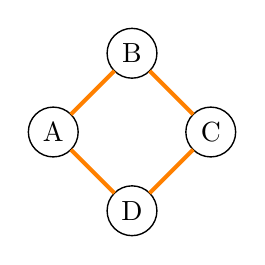
\begin{tikzpicture}
 \SetUpEdge[lw         = 1.5pt,
            color      = orange,
            labelcolor = white]
\tikzset{every node/.style={fill=white}} 
 \tikzset{VertexStyle/.append  style={fill}}
  \Vertex{A}
  \NOEA(A){B}  \SOEA(B){C} \SOEA(A){D}
\tikzset{EdgeStyle/.style={-}} 
\Edge[](A)(B)
  \Edge[](A)(D)
  \Edge[](B)(C)
\Edge[](C)(D)
\end{tikzpicture}
    \end{tabular}
  \end{table}
\end{frame}

\begin{frame}{Subgradient Descent}
  \begin{itemize}
    \setlength{\itemsep}{10pt}
  \item Hence the goal is to solve problems of the form:
\begin{align*}
\label{eq:lasso}
& \argmin_{\beta} F(\beta) =  \argmin_{\beta} g(\beta) + h(\beta)
\end{align*}
where $g(\beta)$ is convex and differentiable and $h(\beta)$ is convex, but non-differentiable. 
\item The basic update in a  subgradient algorithm in such a case is
$$
\beta^{k+1} = \beta^{k} - t_k \partial F(\beta^{k})
$$
where $t_{k}$ is the step size and $\partial F(\beta)$ is the subgradient of $F(\beta)$
  \end{itemize}
\end{frame}

\begin{frame}{What is a subgradient?}
  \begin{itemize}
    \setlength{\itemsep}{10pt}
  \item Recall that a gradient of {\bf differentiable} $F:\mathbb{R}^n \to \mathbb{R}$ at $\beta$ satisfies for all $\eta \in \mathbb{R}^n$ 
$$
F(\eta) \geq F(\beta) + \nabla F(\beta) ^t(\eta - \beta)
$$
  \item A subgradient of convex $F:\mathbb{R}^n \to \mathbb{R}$ at $\beta$ is any $g \in \mathbb{R^n}$ such that for all $\eta \in \mathbb{R}^n$ we have
$$
F(\eta) \geq F(\beta) + g^t(\eta - \beta)
$$
\item If $F$ is differentiable, $g = \nabla F$
\item When $h(\beta) = \norm{\beta}_1$, the subgradient is equal to $s$, where
$$
s_i = \begin{cases}
\sign(\beta_i) &\text{ if } \beta_i \neq 0\\
[-1,1] &\text{ if } \beta_i = 0
\end{cases}
$$
  \end{itemize}
\end{frame}

\begin{frame}{Subgradient methods for BP:}
  \begin{itemize}
    \setlength{\itemsep}{10pt}
  \item For the BP problem, the subgradient is $-X^t(y-X\beta) + \lambda s$ with
$$
s_i = \begin{cases}
\sign(\beta_i) &\text{ if } \beta_i \neq 0\\
0 &\text{ if } \beta_i = 0
\end{cases}
$$
\item Hence the basic update is:
$$\beta^k = \beta^{k-1} + t_k (X^t(y-X \beta^{k-1}) - \lambda s^{k-1})$$
\item For back-tracking line search, fix $\eta \in (0,1)$. At each iteration, while 
$$
F(\beta - t \partial F(\beta)) > F(\beta) - \frac{t}{2} \norm{\partial F(\beta)}^2
$$
let $t = \eta t$.
  \end{itemize}
\end{frame}

\begin{frame}{Subgradient methods for Gaussian Graphical Models:}
  \begin{itemize}
    \setlength{\itemsep}{10pt}
  \item For the $glasso$ problem, the subgradient is $ S - \Omega^{-1} + \lambda \Gamma$ with
$$
\Gamma_{ij} = \begin{cases}
\sign(\Omega_{ij}) &\text{ if } \Omega_{ij ,i \neq j} \neq 0\\
0 &\text{ if } \Omega_{ij} = 0, \Omega_{ij, i = j}
\end{cases}
$$
\item Hence the basic update is:
$$\Omega^k = \Omega^{k-1} + t_k ( S - (\Omega^{k-1})^{-1} + \lambda \Gamma^{k-1})$$
  \end{itemize}
\end{frame}

\begin{frame}{Convergence of subgradient methods:}
\begin{thm}
For fixed step sizes, the sudgradient method satisfies 
$$
\lim_{k \to \infty} F(\beta^k) \leq F(\beta^*) + \frac{L^2t}{2}
$$
with convergenve rate of $O(\frac{1}{\sqrt{k}})$.
\end{thm}
where $\abs{F(\beta^1) - F(\beta^2)} \leq L \norm{\beta^1 - \beta^2}$

\begin{thm}
For diminshing step sizes, the sudgradient method satisfies 
$$
\lim_{k \to \infty} F(\beta^k) = F(\beta^*)
$$
with convergenve rate of $O(\frac{1}{\sqrt{k}})$.
\end{thm}
\end{frame}

\begin{frame}{Proximal Gradient Methods:}
  \begin{itemize}
    \setlength{\itemsep}{10pt}
\item The prioximal operator for $h(\beta)$ is: \begin{align*}
\text{prox}_t(\beta) &= \argmin_{\eta} \frac{1}{2t} \norm{\beta-\eta}_2^2 + h(\eta)
\end{align*}
  \item The proximal gradient method to minimize $F(\beta) = g(\beta) + h(\beta)$ is:
\begin{align*}
\beta^{(k)} = \text{prox}_{t_kh}(\beta^{(k-1)}-t_k \nabla g(\beta^{(k-1)}))
\end{align*}
\item To see why this works, note that
\begin{align*}
\beta^+ &= \argmin_{\eta} (h(\eta) + \frac{1}{2t} \norm{\eta - \beta + t \nabla g(\beta)}_2^2) \\
&= ...\\
&= \argmin_{\eta} (h(\eta) + g(\beta) + \nabla g(\beta)^t(\eta - \beta) + \frac{1}{2t} \norm{\eta - \beta}_2^2) 
\end{align*}
  \end{itemize}
\end{frame}

\begin{frame}{How Proximal Gradient methods work:}
  \begin{itemize}
    \setlength{\itemsep}{10pt}
\item Recall, the $2^{nd}$ order Taylor series approximation to $g(\eta)$ near $\beta$ is 
\begin{align*}
g(\eta) =& g(\beta) + \nabla g(\beta)^t (\eta - \beta) + (\eta-\beta)^t \nabla^2 g(\beta) (\eta -\beta) \\
&\leq  g(\beta) + \nabla g(\beta)^t (\eta - \beta) + L (\eta-\beta)^t (\eta -\beta)
\end{align*}
where the function $\nabla g(\beta)$ has Lipschitz constant $L$.
\item Hence, we are essentially minimizing $h(\eta)$ plus a simple local model of $g(\eta)$ around $\beta$.
  \end{itemize}
\end{frame}

\begin{frame}{ISTA for BP:}
  \begin{itemize}
    \setlength{\itemsep}{10pt}
\item The proximal operator for the $\ell_1$
penalty, $h(\beta) = \lambda \norm{\beta}_1$ is 
\begin{align*}
\text{prox}_t(\beta) 
&= \argmin_{\eta} \frac{1}{2t} \norm{\beta-\eta}_2^2 +
  \lambda \norm{\eta}_1 \\
 &= S_{\lambda t} (\beta)
\end{align*}
where $[S_{\lambda t} (\beta)]_i = \sign (x_i)* \max\{ \abs{\beta_i} - \lambda
t, 0 \}$
\item In addition, $\nabla g(\beta) = -X^t (y -
X \beta)$
\item Hence the ISTA update is:
\begin{align*}
\beta^{k} = S_{\lambda t_k} (\beta^{k-1} + t_k X^t (y -
X \beta^{k-1})) 
\end{align*}
  \end{itemize}
\end{frame}

\begin{frame}{Choice of step-size:}
  \begin{itemize}
    \setlength{\itemsep}{10pt}
\item Note that for BP, we have that 
\begin{align*}
\norm{\nabla g(\beta_1) - \nabla g(\beta_2)}_2 & \leq L \norm{\beta_1 - \beta_2}_2 \\
&= \lambda_{max}(X^t X) \norm{\beta_1 - \beta_2}_2
\end{align*}
\item Hence set $t_k = 1/L$
\item If $L$ is difficult to attain, use back-tracking line-search
  \end{itemize}
\end{frame}

\begin{frame}{FISTA for BP:}
  \begin{itemize}
    \setlength{\itemsep}{10pt}
\item In 1983, Nesterov proposed the following Accelarated gradient descent algorithm for convex, differentiable functions $g(\beta)$:
\begin{align*}
\beta^{k+1} = \eta^{k} - t_k \nabla g(\eta^k) \\
\eta^{k+1} = (1- \gamma_k) \beta^{k+1} + \gamma_k \beta^{k}
\end{align*}
with convergence rate $O(\frac{1}{k^2})$.
\item FISTA is essentially this method combined with ISTA. The basic updates are as follows:
\begin{align*}
t_{k+1} &= \frac{1 + \sqrt{1+4t_k^2}}{2} \\
\gamma &= \beta^{k-1} + \frac{t_k-1}{t_{k+1}} (\beta^{k-1} - \beta^{k-2}) \\
\beta^{k} &= S_{\lambda t_k} (\gamma + t_k X^t (y -
X \gamma)) 
\end{align*}
  \end{itemize}
\end{frame}

\begin{frame}{ISTA/FISTA for Gaussian Graphical Models:}
  \begin{itemize}
    \setlength{\itemsep}{10pt}
\item Recall that we want to minimize
\begin{equation*} 
\hat{\Omega} = \argmin_{\Omega \succ 0} (\trace (\Omega S)-\log |\Omega| + \lambda \norm{\Omega}_1)
\end{equation*}
\item Now $\nabla (\trace (\Omega S)-\log |\Omega|) = S - \Omega^{-1}$ 
\item Hence the basic graphical-ISTA update is:
\begin{align*}
\Omega^{k+1} = S_{\lambda t_k}(\Omega^{k} + t_k (S - (\Omega^{k})^{-1}))
\end{align*}
\item And the basic graphical-FISTA update is:
\begin{align*}
\Omega^{k+1} = S_{\lambda t_k}(\zeta^{k} + t_k (S-(\zeta^{k})^{-1})) \\
t_{k+1} = \frac{1 + \sqrt{1+4t_k^2}}{2}\\
\zeta^{k} = \Omega^{k+1} + \frac{t_k-1}{t_{k+1}}(\Omega^{k+1}  - \Omega^{k} )
\end{align*}
  \end{itemize}
\end{frame}

\begin{frame}{Convergence for ISTA/FISTA:}
\begin{thm}
Let $\beta^k$ be a sequence generated by either of the ISTA algorithms as described above. Then for any $k\geq 1$
$$
F(\beta_k) - F(\beta^*) \leq \frac{\alpha L(g) \norm{\beta_0 - \beta^*}_2}{2k}
$$
where $\alpha = 1$ for constant step size and $\alpha = \eta$ for back-tracking line search.
\end{thm}

\begin{thm}
Let $\beta^k$ be a sequence generated by either of the FISTA algorithms as described above. Then for any $k\geq 1$
$$
F(\beta_k) - F(\beta^*) \leq \frac{\alpha L(g) \norm{\beta_0 - \beta^*}_2}{(k+1)^2}
$$
where $\alpha = 1$ for constant step size and $\alpha = \eta$ for back-tracking line search.
\end{thm}
\end{frame}

\begin{frame}{ADMM for BP:}
  \begin{itemize}
    \setlength{\itemsep}{10pt}
\item ADMM mixes the decomposability of the \textit{dual ascent method} with the superior convergence properties of the \textit{method of multipliers}. 
\item Recall the BP problem:
\begin{align*}
\frac{1}{2}\norm{y- X \beta}_2^2 + \lambda
  \norm{\beta}_1 
\end{align*}
\item This is equivalent to:
\begin{align*}
\frac{1}{2}\norm{y- X \beta}_2^2 + \lambda
  \norm{\gamma}_1 \text{ s.t. } \beta = \gamma
\end{align*}
\item The augmented Lagrangian in this case is: 
\begin{align*}
 \frac{1}{2}\norm{y- X \beta}_2^2 + \lambda
  \norm{\gamma}_1 + \frac{\rho}{2} \norm{\beta - \gamma}_2^2 \text{ s.t. } \beta = \gamma
\end{align*}
  \end{itemize}
\end{frame}

\begin{frame}{ADMM for BP continued:}
  \begin{itemize}
    \setlength{\itemsep}{10pt}
\item We can rewrite this as:
\begin{align*}
L(\beta, \gamma, \eta) = \frac{1}{2}\norm{y- X \beta}_2^2 + \lambda
  \norm{\gamma}_1 + \frac{\rho}{2} \norm{\beta - \gamma}_2^2 + \eta^t(\beta - \gamma)
\end{align*}
\item To minimize this we need to following updates:
\begin{align*}
\beta^{k} = \argmin_\beta L(\beta^{k-1}, \gamma, \eta)\\
\gamma^{k} = \argmin_\gamma L(\beta, \gamma^{k-1}, \eta)\\
\eta^{k} = \eta^{k-1}+ \rho(\beta - \gamma)\\
\end{align*}
where the last step is the \textit{dual ascent step}
  \end{itemize}
\end{frame}

\begin{frame}{Convergence for ADMM:}
  \begin{itemize}
    \setlength{\itemsep}{10pt}
\item Define $r^k = \beta^k - \eta^k$. Then $r^k \to 0$ as $k \to \infty$
\item $\frac{1}{2}\norm{y- X \beta^k}_2^2 + \lambda
  \norm{\gamma^k}_1 \to p^*$ as $k \to \infty$ where $p^*$ is the optimal value 
\item $\eta^k \to \eta^*$ as $k \to \infty$ where $\eta^*$ is a dual optimal point
  \end{itemize}
\end{frame}

\begin{frame}{ADMM for Gaussian Graphical Models:}
  \begin{itemize}
    \setlength{\itemsep}{10pt}
\item Recall that we want to solve:
$$
\min_{\Omega \succ 0} \trace(S\Omega) - \log \abs{\Omega} + \lambda \norm{\Omega}_1
$$
\item This is equivalent to:
\begin{align*}
&\min_{\Omega,Z} \trace(S\Omega) - \log \abs{\Omega} + \lambda \norm{Z}_1 \text{ s.t } \Omega = Z 
\end{align*}
\item The augmented Lagrangian in this case is:
\begin{align*}
&\min_{\Omega,Z,Y} \trace(S\Omega) - \log \abs{\Omega} + \lambda \norm{Z}_1 + Y^t (\Omega - Z) + \frac{\rho}{2} \norm{\Omega-Z}_F^2
\end{align*}
  \end{itemize}
\end{frame}

\begin{frame}{ADMM for Gaussian Graphical Models:}
  \begin{itemize}
    \setlength{\itemsep}{10pt}
\item Solving this involves doing the following at each iteration:
\begin{align*}
\min_{\Omega} \trace(S\Omega) - \log \abs{\Omega} + Y^t (\Omega - Z) + \frac{\rho}{2} \norm{\Omega-Z}_F^2\\
\min_{Z}  \lambda \norm{Z}_1 + Y^t (\Omega - Z) + \frac{\rho}{2} \norm{\Omega-Z}_F^2 \\
\max_{Y}  Y^t (\Omega - Z) 
\end{align*}
  \end{itemize}
\end{frame}

\begin{frame}{Data for BP Experiments:}
  \begin{itemize}
    \setlength{\itemsep}{10pt}
\item We set $p = 200$ and $n = \{20,50,100,500\}$.
\item Number of non-zero elements of $\beta^*$ was set equal to $20$. 
\item $X_{ij} \overset{iid}{\sim} \mathcal{N}(0,1); i = 1,...,n; j = 1,...,p$, $E_{i} \overset{iid}{\sim} \mathcal{N}(0,1); i = 1,...,n$ and $y = X\beta^* + E$.
\item $\lambda$ was picked through 5-fold cross-validation
\item We compared $\norm{\beta^k - \beta^{k-1}}_\infty$ at each step, timing and $\frac{\norm{\hat{\beta}-\beta^*}_2^2}{\norm{\beta^*}_2^2}$ for all the methods
\item In the above case, $X$ had a condition number of $3.1677$. We repeated the experiments with with X having a condition number of $101.9279$. The performance of the subgradient method was very poor showing how this algorithm lacks stability. ISTA/FISTA's performance was pretty good, but inconsistent. The most reilable was the ADMM algorithm, whose performance hardly changed.   
  \end{itemize}
\end{frame}

\begin{frame}{Convergence Plots for Basis Pursuit:}
\fontsize{6pt}{7.2}\selectfont
\begin{figure}[H]
  \centering
    \begin{subfigure}[b]{0.2\textwidth}
        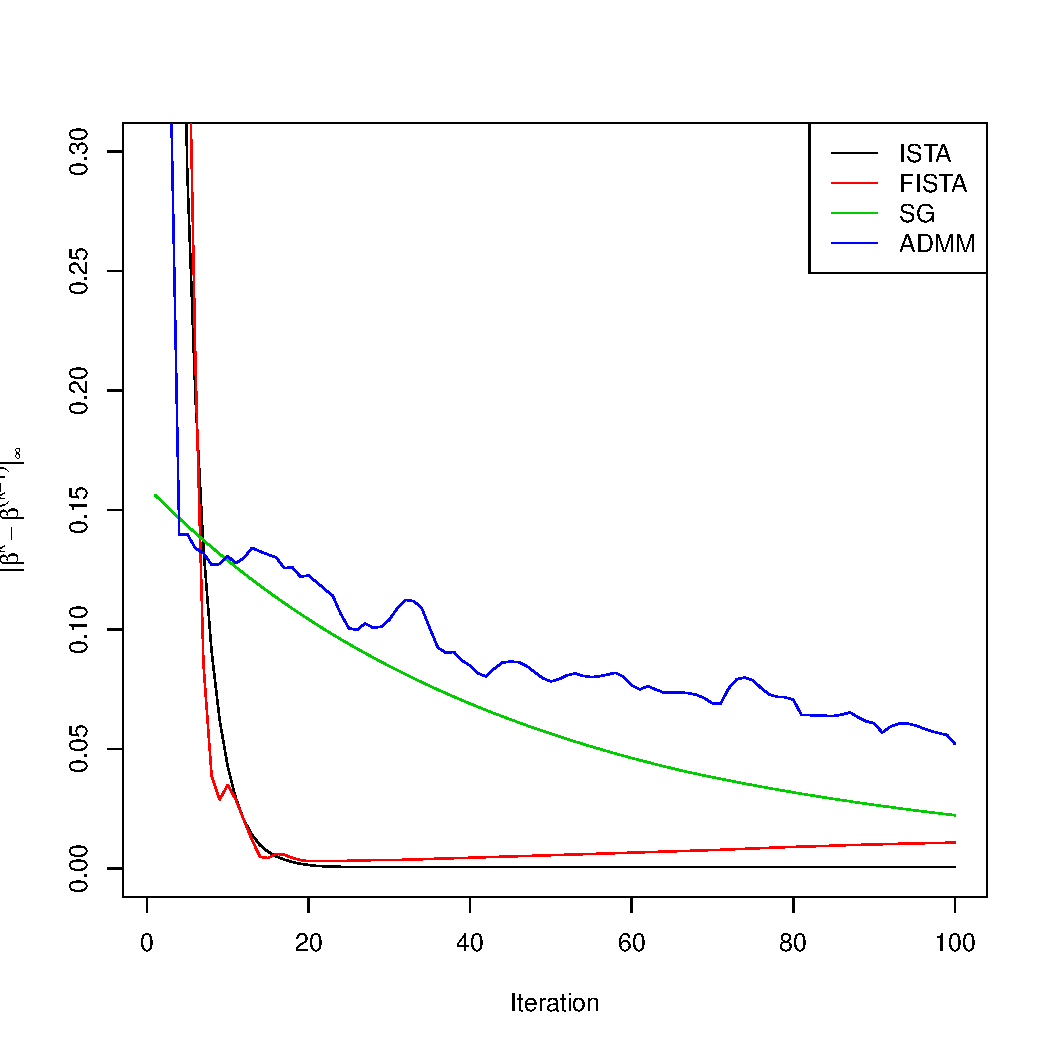
\includegraphics[width=\textwidth]{20cvgc.pdf}
        \caption{$n=20$}
        \label{fig:20}
    \end{subfigure}
~
    \begin{subfigure}[b]{0.2\textwidth}
        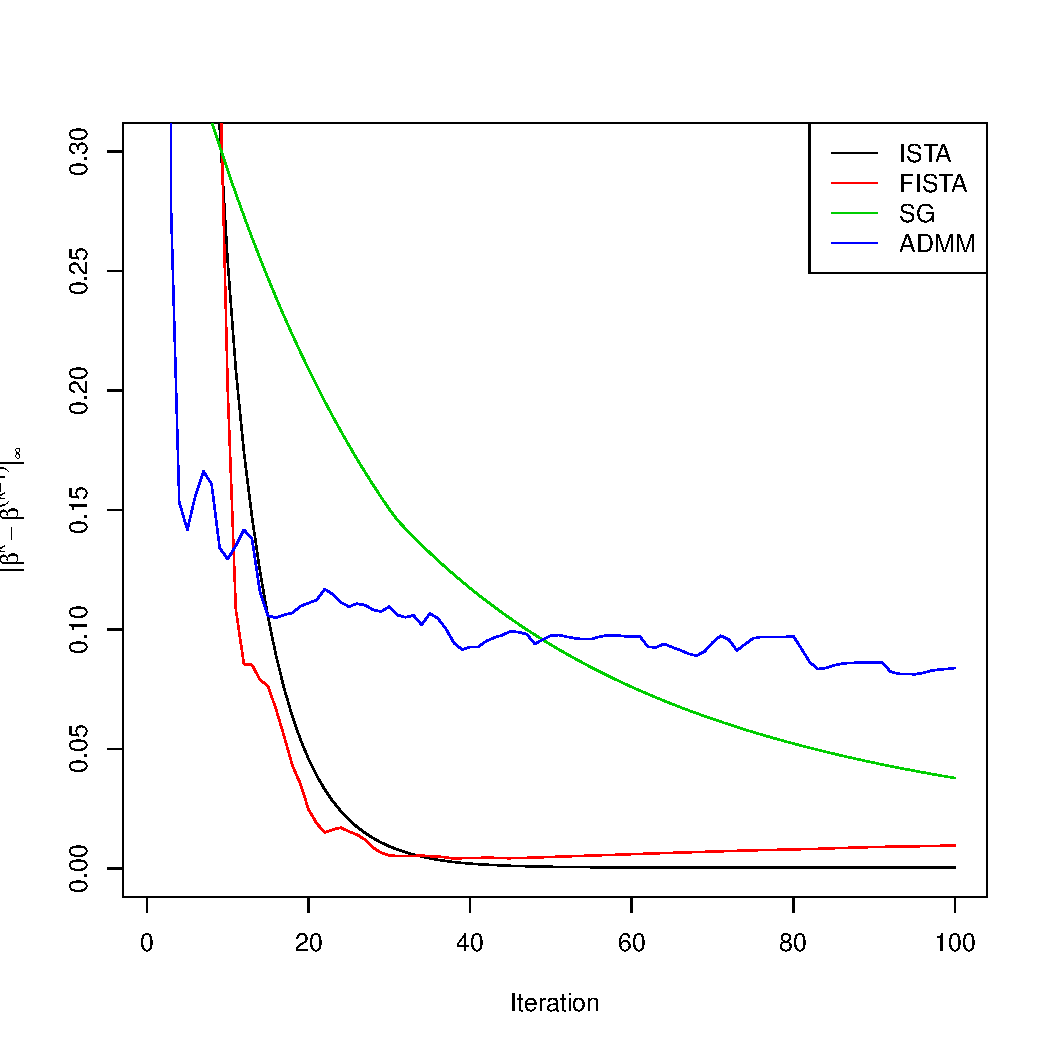
\includegraphics[width=\textwidth]{50cvgc.pdf}
        \caption{$n=50$}
        \label{fig:50}
    \end{subfigure}
\\
    \begin{subfigure}[b]{0.2\textwidth}
        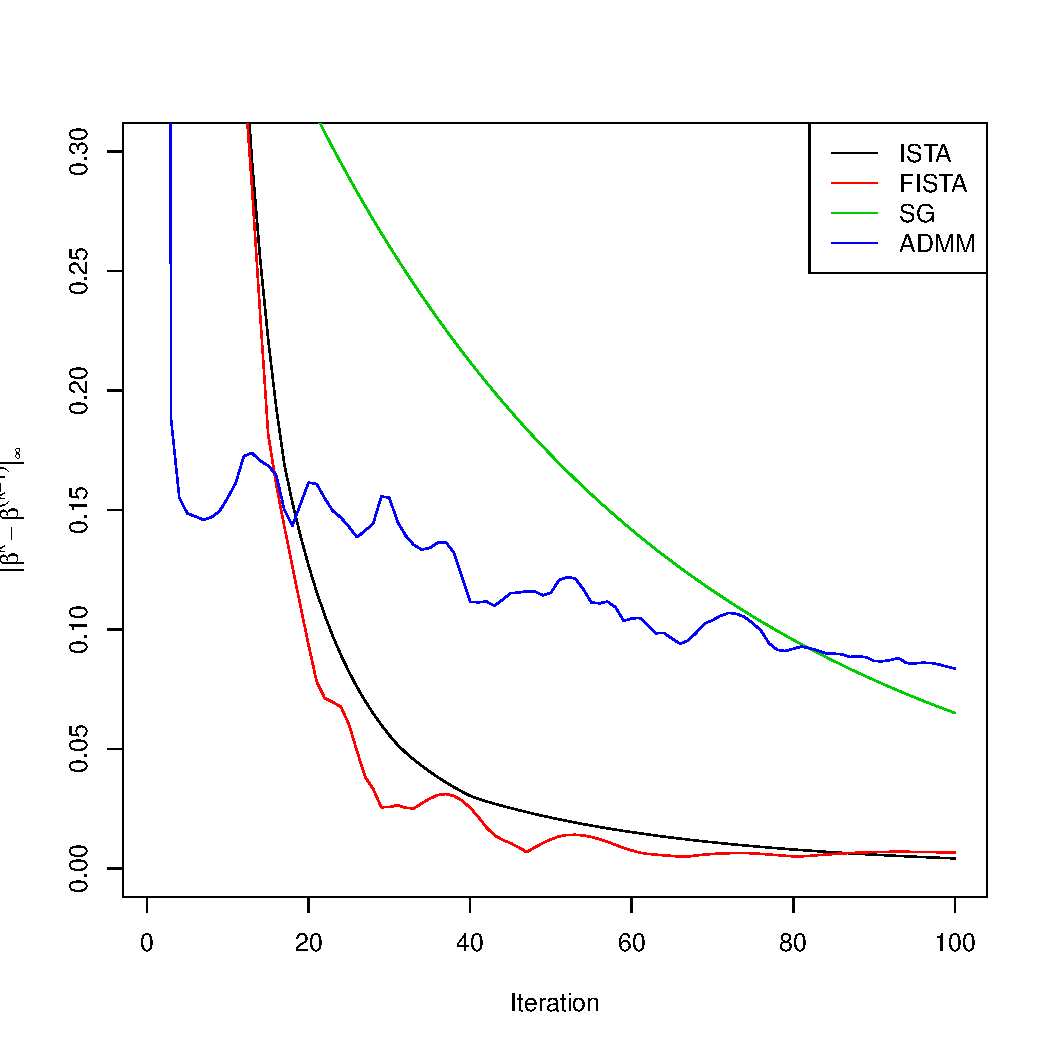
\includegraphics[width=\textwidth]{100cvgc.pdf}
        \caption{$n=100$}
        \label{fig:100}
    \end{subfigure}
~
    \begin{subfigure}[b]{0.2\textwidth}
        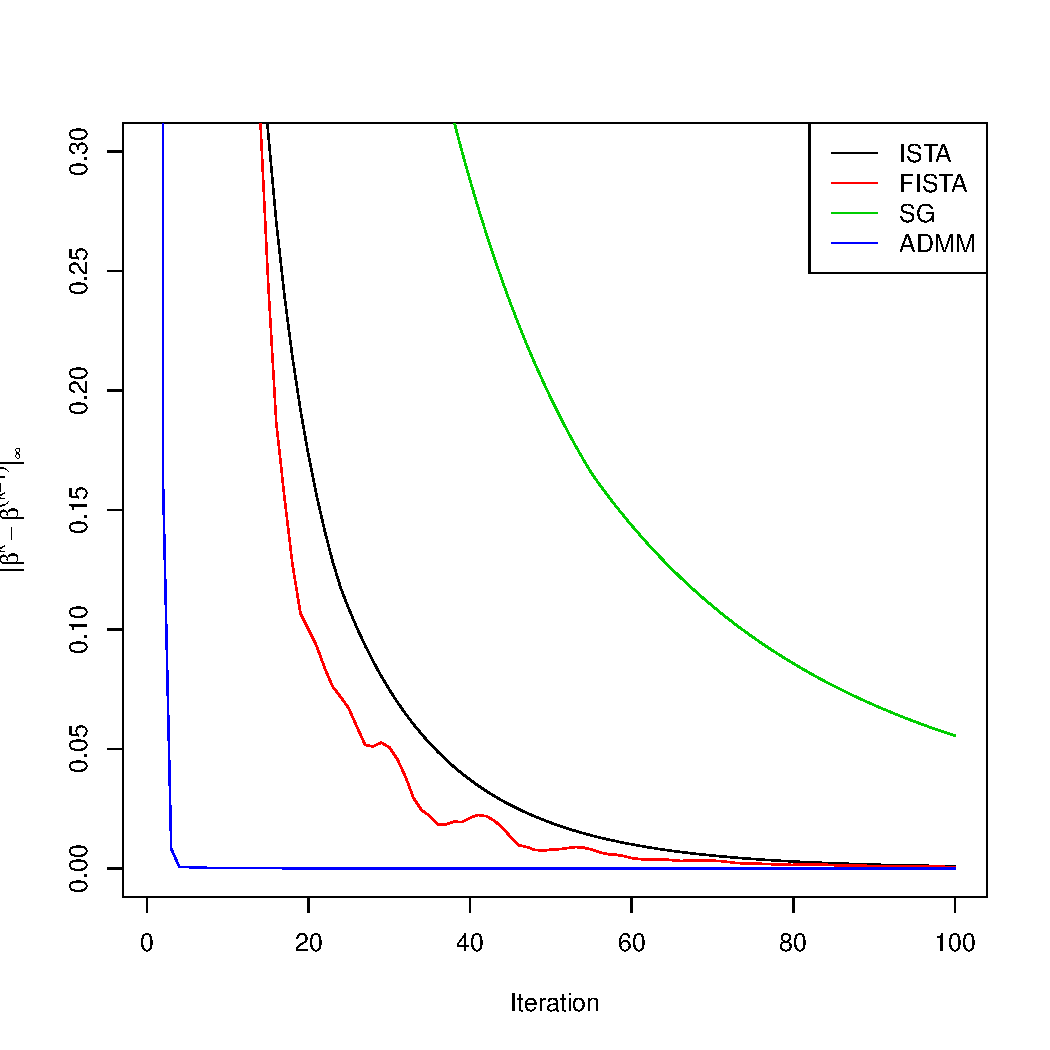
\includegraphics[width=\textwidth]{500cvgc.pdf}
        \caption{$n=500$}
        \label{fig:500}
    \end{subfigure}
\label{fig:cvgc}
\end{figure}
\end{frame}

\begin{frame}{Timing plots for Basis Pursuit:}
\fontsize{6pt}{7.2}\selectfont
\begin{figure}[H]
  \centering
    \begin{subfigure}[b]{0.2\textwidth}
        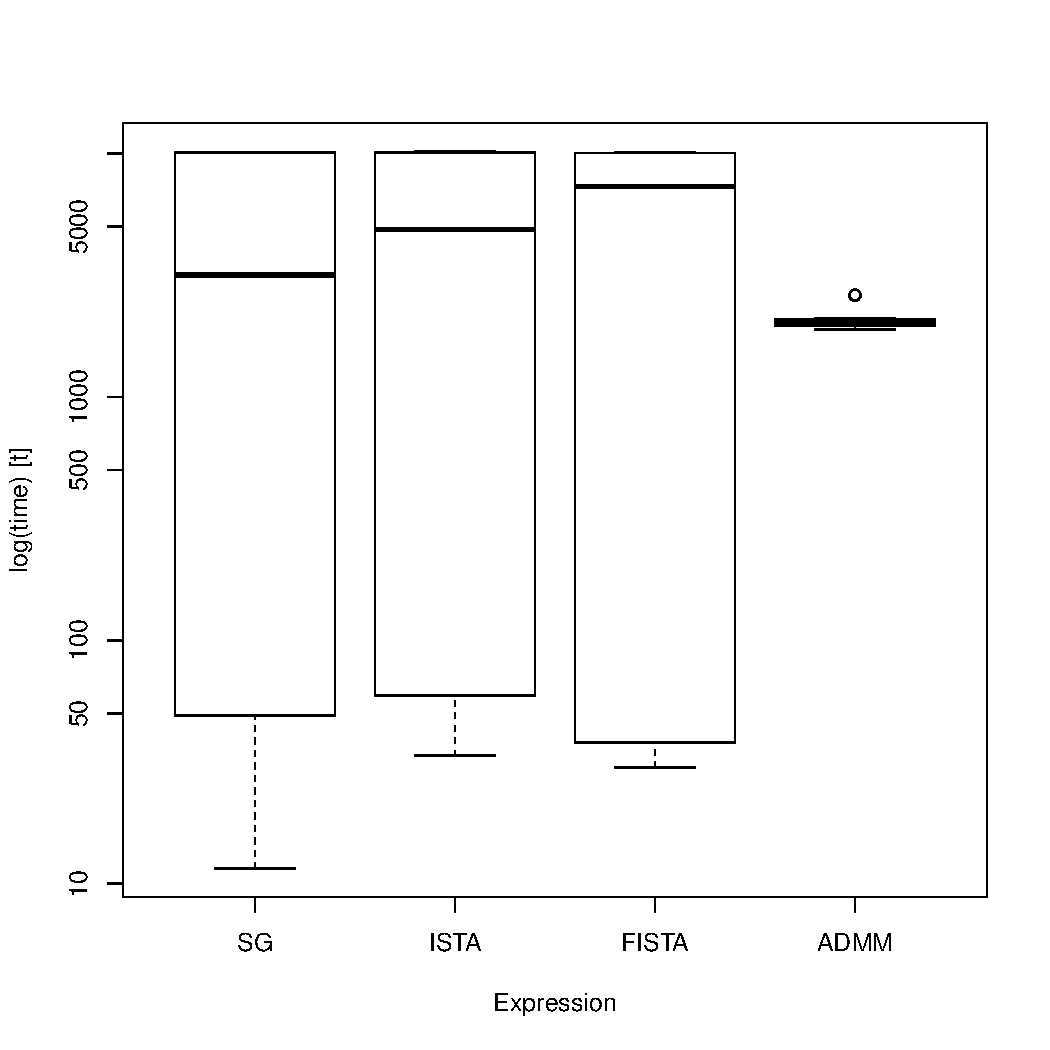
\includegraphics[width=\textwidth]{20timing.pdf}
        \caption{$n=20$}
        \label{fig:20}
    \end{subfigure}
~
    \begin{subfigure}[b]{0.2\textwidth}
        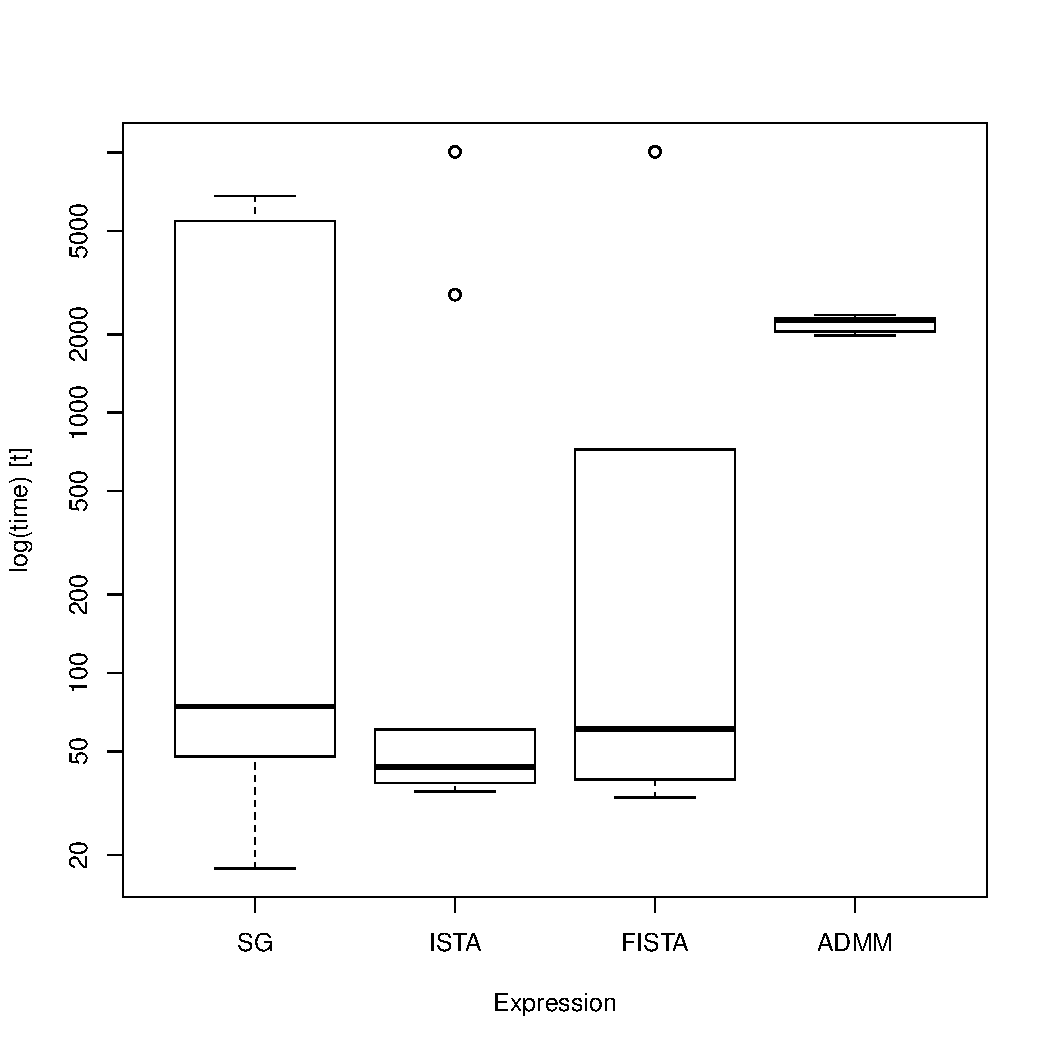
\includegraphics[width=\textwidth]{50timing.pdf}
        \caption{$n=50$}
        \label{fig:50}
    \end{subfigure}
\\
    \begin{subfigure}[b]{0.2\textwidth}
        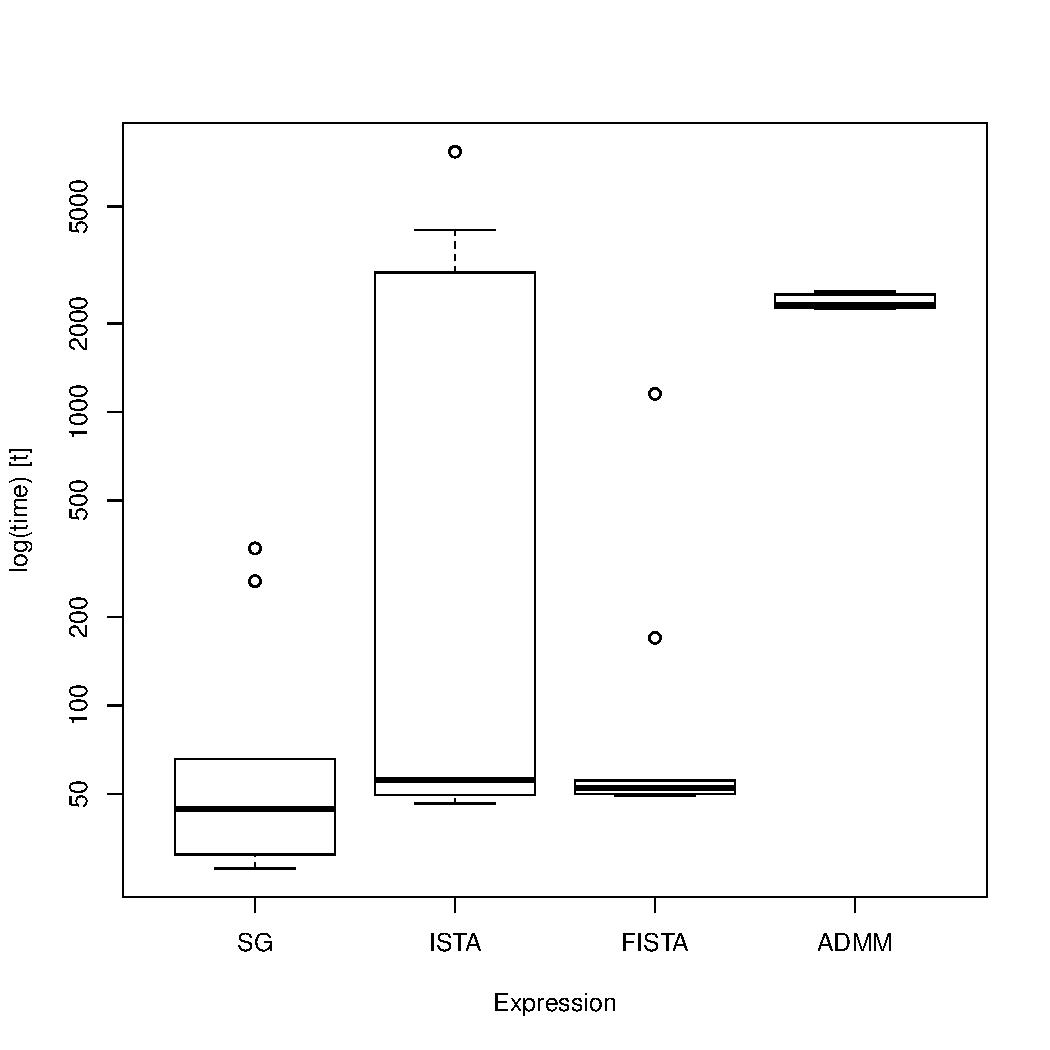
\includegraphics[width=\textwidth]{100timing.pdf}
        \caption{$n=100$}
        \label{fig:100}
    \end{subfigure}
~
    \begin{subfigure}[b]{0.2\textwidth}
        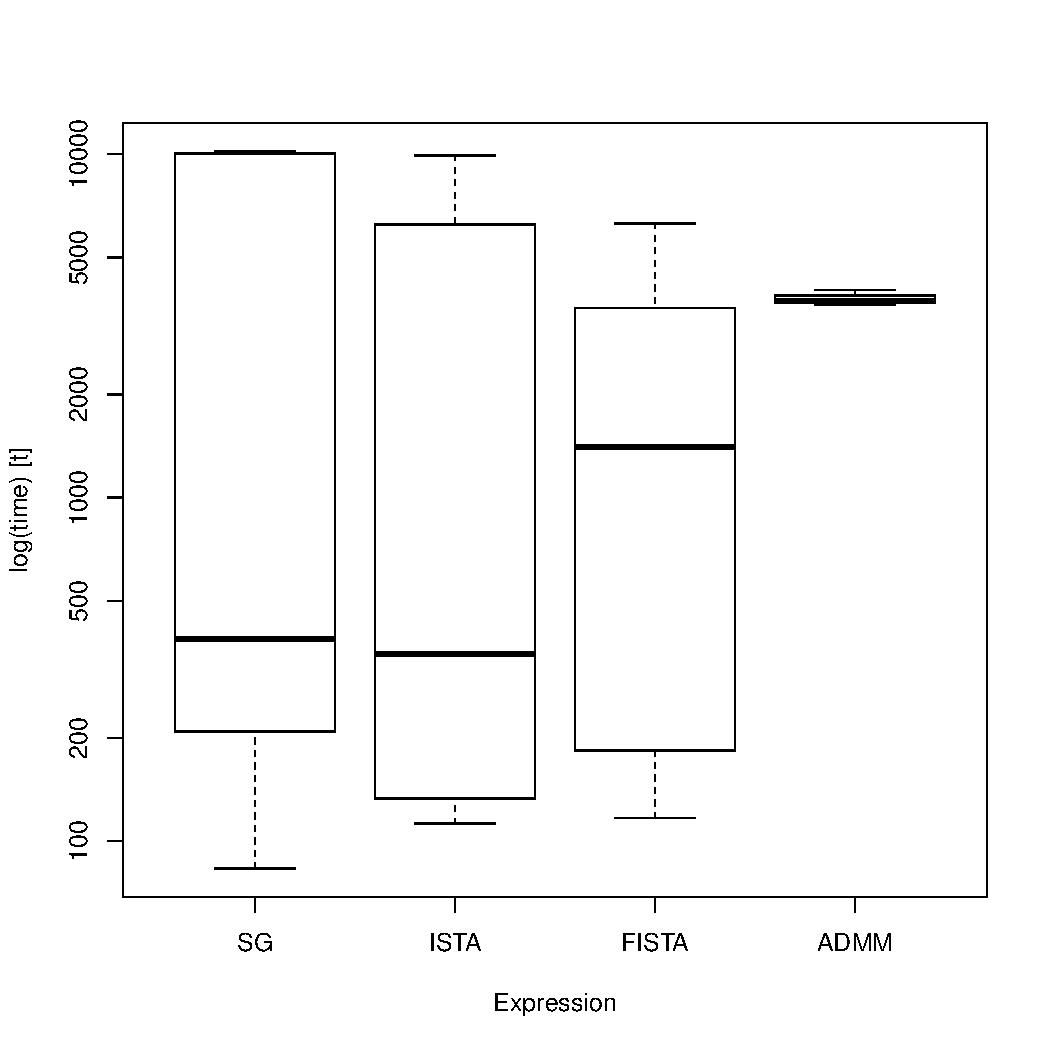
\includegraphics[width=\textwidth]{500timing.pdf}
        \caption{$n=500$}
        \label{fig:500}
    \end{subfigure}
\label{fig:cvgc}
\end{figure}
\end{frame}

\begin{frame}{Relative Norm Error ($\frac{\norm{\hat{\beta}-\beta^*}_2^2}{\norm{\beta^*}_2^2}$):}
\begin{table}[ht]
\centering
\begin{tabular}{rlrrrr}
  \hline
 & Method & $n=20$ & $n=50$ & $n=100$ & $n=500$ \\ 
  \hline
1 & SG & 0.0184 & 0.0164 & 0.0095 & 0.0007\\ 
  2 & ISTA& 0.0188 & 0.0146 & 0.0036 & 0.00008\\ 
  3 & FISTA & 0.0197 & 0.0149 & 0.0038 & 0.00008\\ 
  4 & ADMM & 0.0223 & 0.0174 & 0.0053 & 0.00008\\ 
   \hline
\end{tabular}
\label{tab:relnorm}
\end{table}
\end{frame}

\begin{frame}{Convergence Plots for Basis Pursuit for ill-conditioned X:}
\fontsize{6pt}{7.2}\selectfont
\begin{figure}[H]
  \centering
    \begin{subfigure}[b]{0.2\textwidth}
        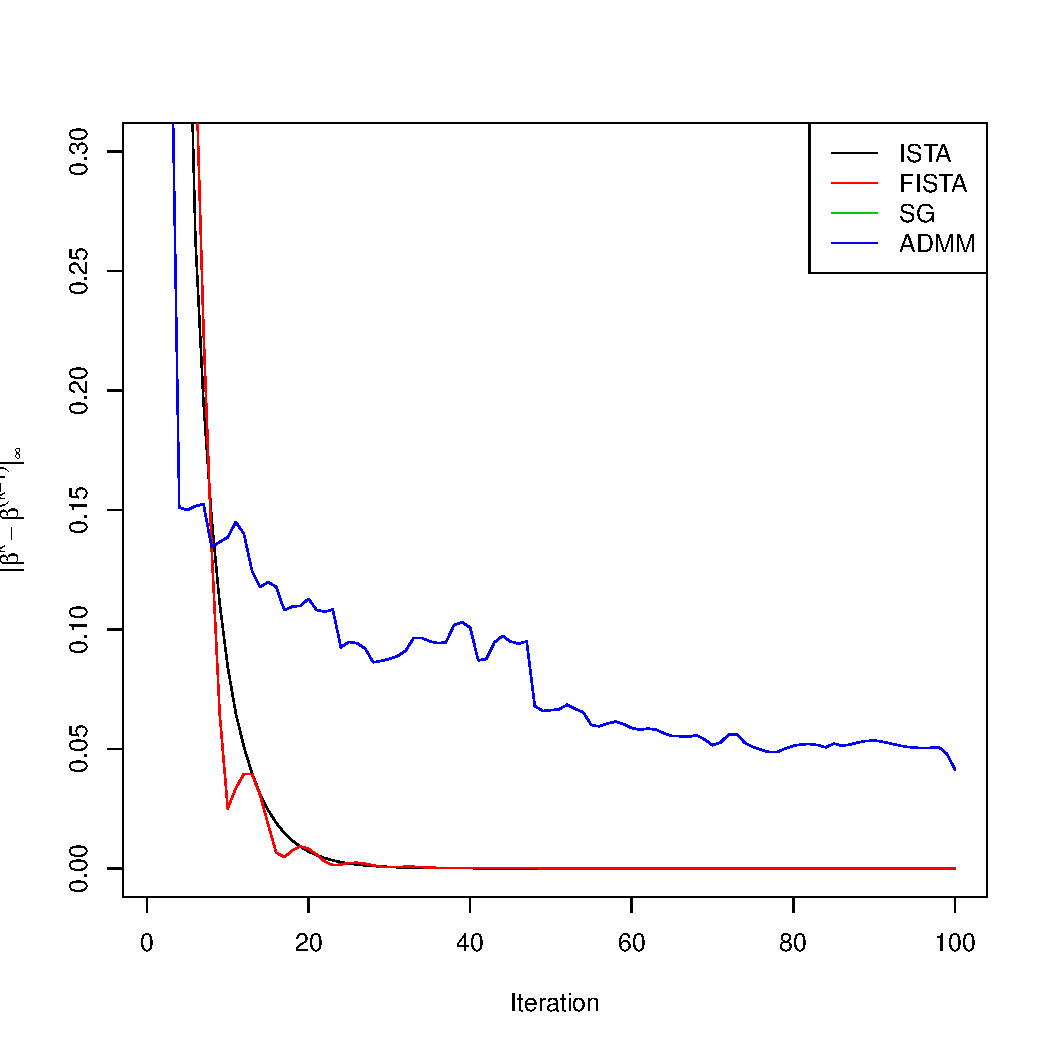
\includegraphics[width=\textwidth]{20cvgc-cn.pdf}
        \caption{$n=20$}
        \label{fig:20}
    \end{subfigure}
~
    \begin{subfigure}[b]{0.2\textwidth}
        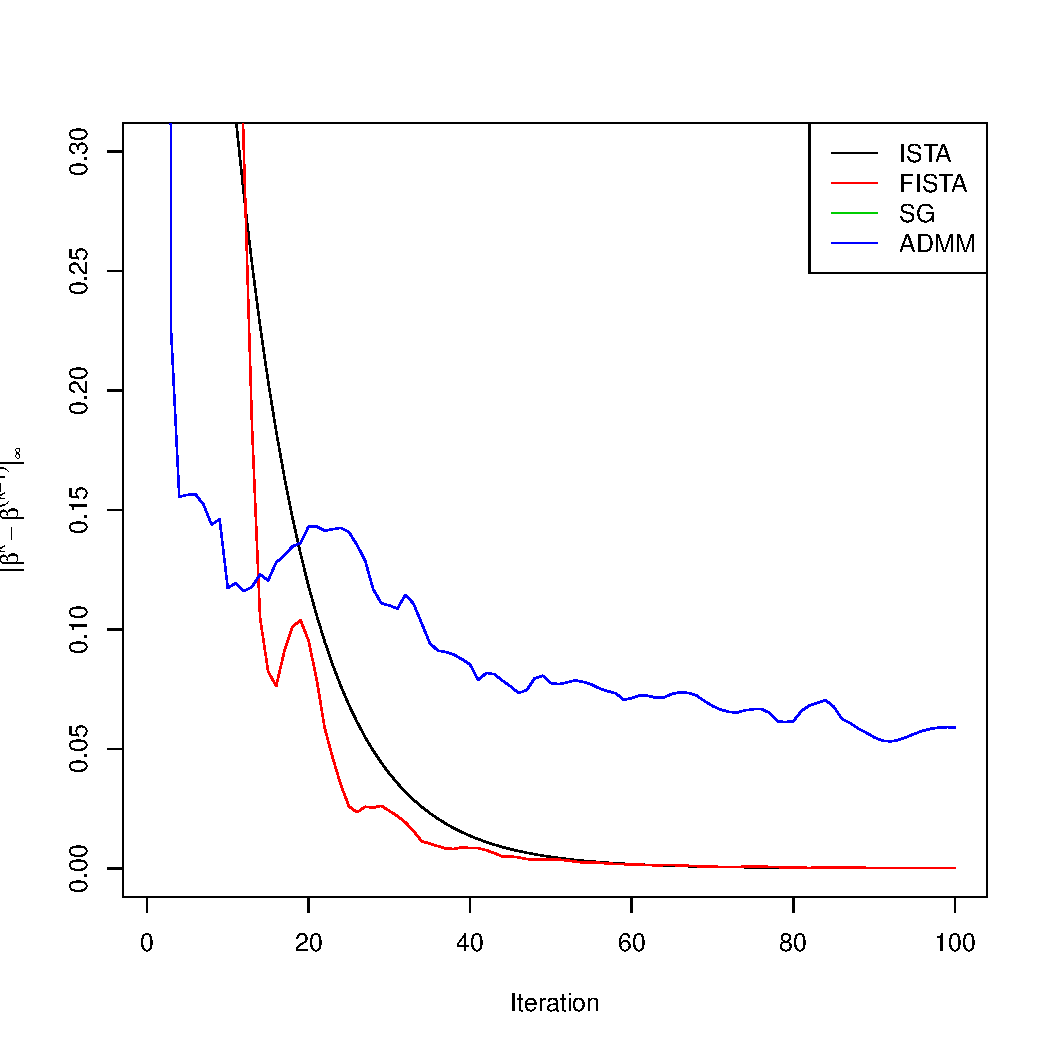
\includegraphics[width=\textwidth]{50cvgc-cn.pdf}
        \caption{$n=50$}
        \label{fig:50}
    \end{subfigure}
\\
    \begin{subfigure}[b]{0.2\textwidth}
        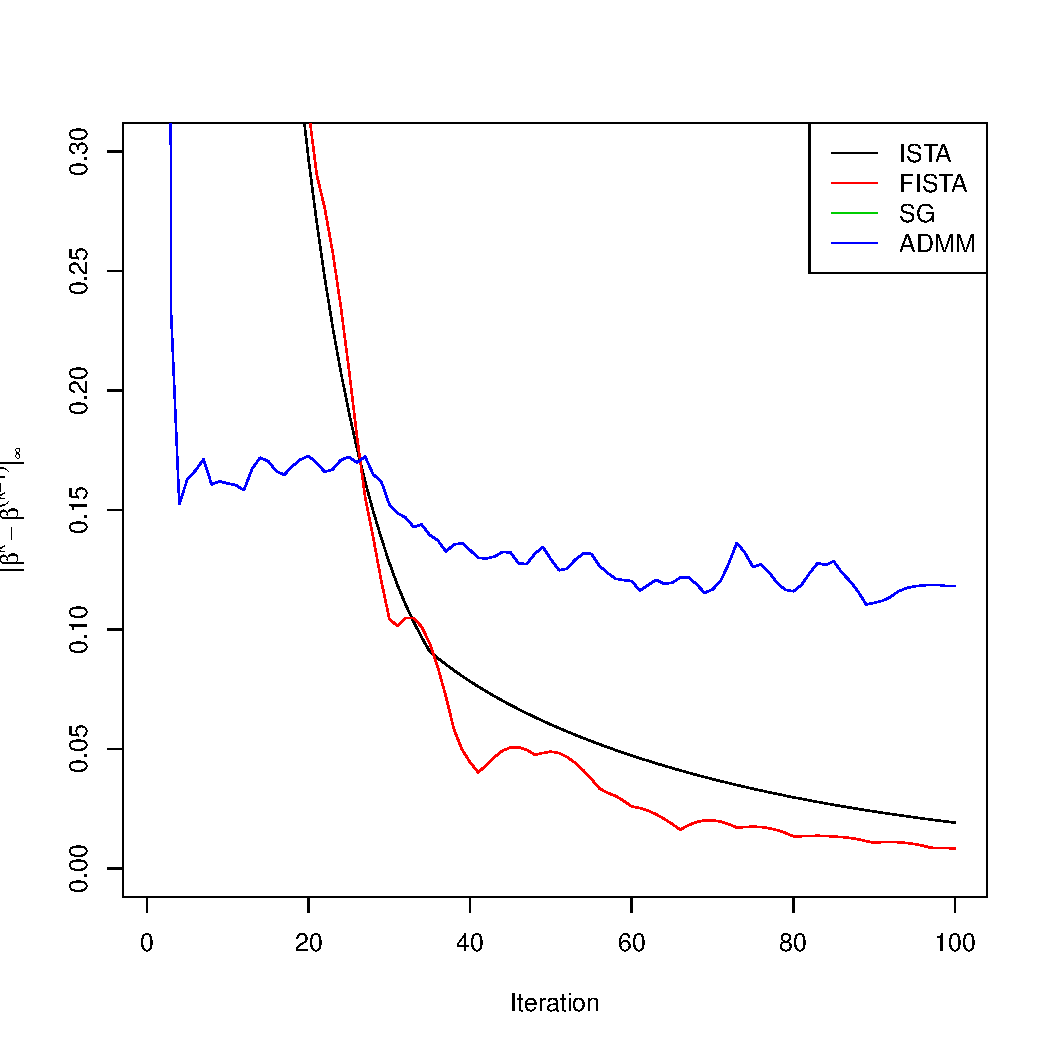
\includegraphics[width=\textwidth]{100cvgc-cn.pdf}
        \caption{$n=100$}
        \label{fig:100}
    \end{subfigure}
~
    \begin{subfigure}[b]{0.2\textwidth}
        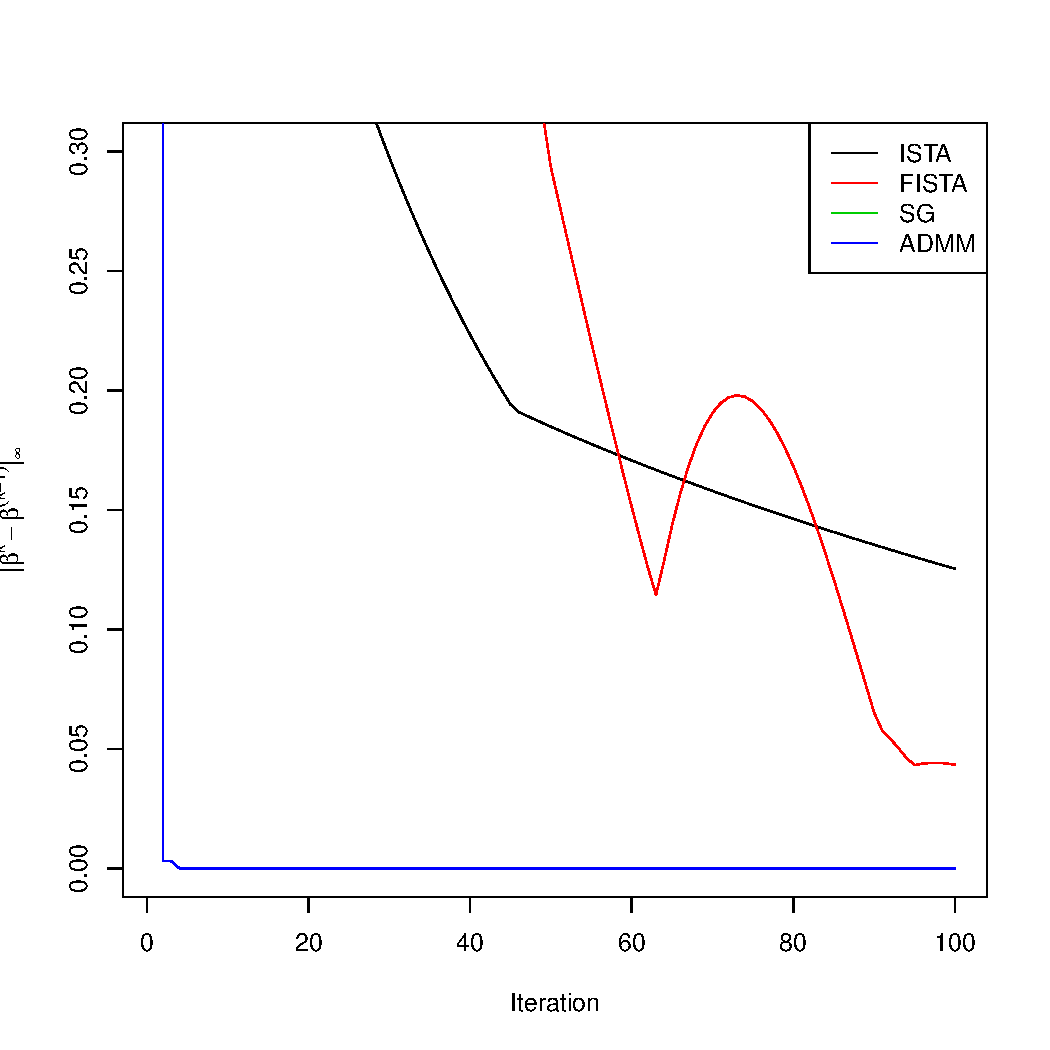
\includegraphics[width=\textwidth]{500cvgc-cn.pdf}
        \caption{$n=500$}
        \label{fig:500}
    \end{subfigure}
\label{fig:cvgc}
\end{figure}
\end{frame}

\begin{frame}{Timing plots for Basis Pursuit for ill-conditioned X:}
\fontsize{6pt}{7.2}\selectfont
\begin{figure}[H]
  \centering
    \begin{subfigure}[b]{0.2\textwidth}
        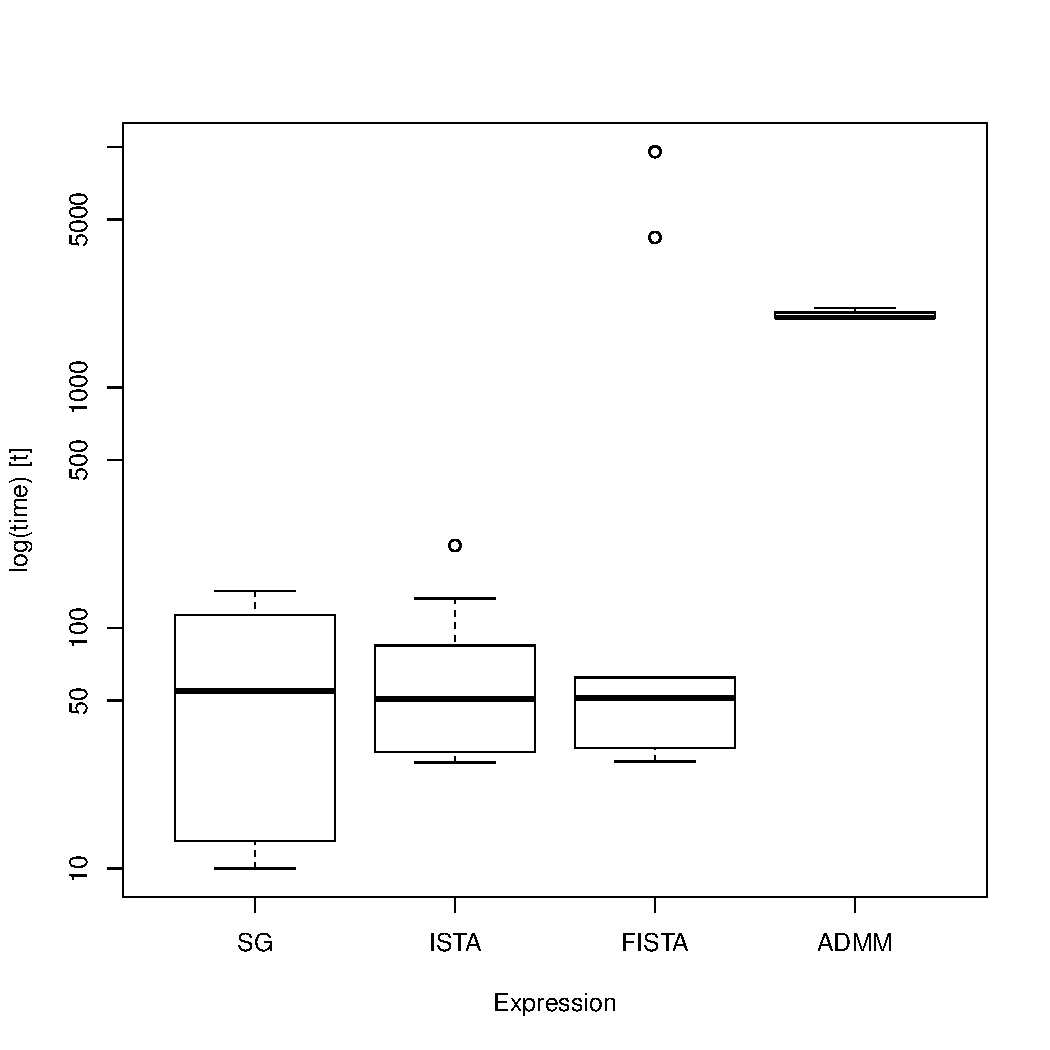
\includegraphics[width=\textwidth]{20timing-cn.pdf}
        \caption{$n=20$}
        \label{fig:20}
    \end{subfigure}
~
    \begin{subfigure}[b]{0.2\textwidth}
        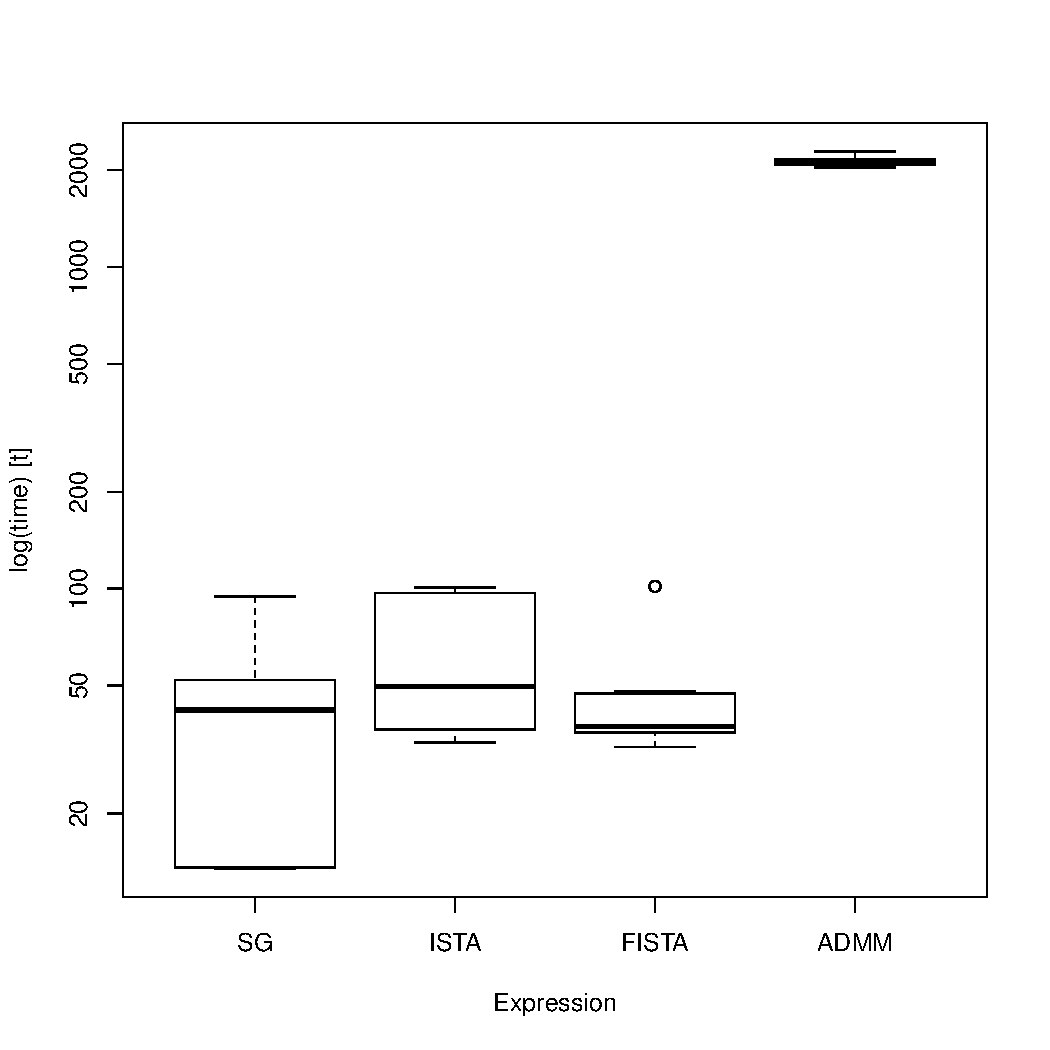
\includegraphics[width=\textwidth]{50timing-cn.pdf}
        \caption{$n=50$}
        \label{fig:50}
    \end{subfigure}
\\
    \begin{subfigure}[b]{0.2\textwidth}
        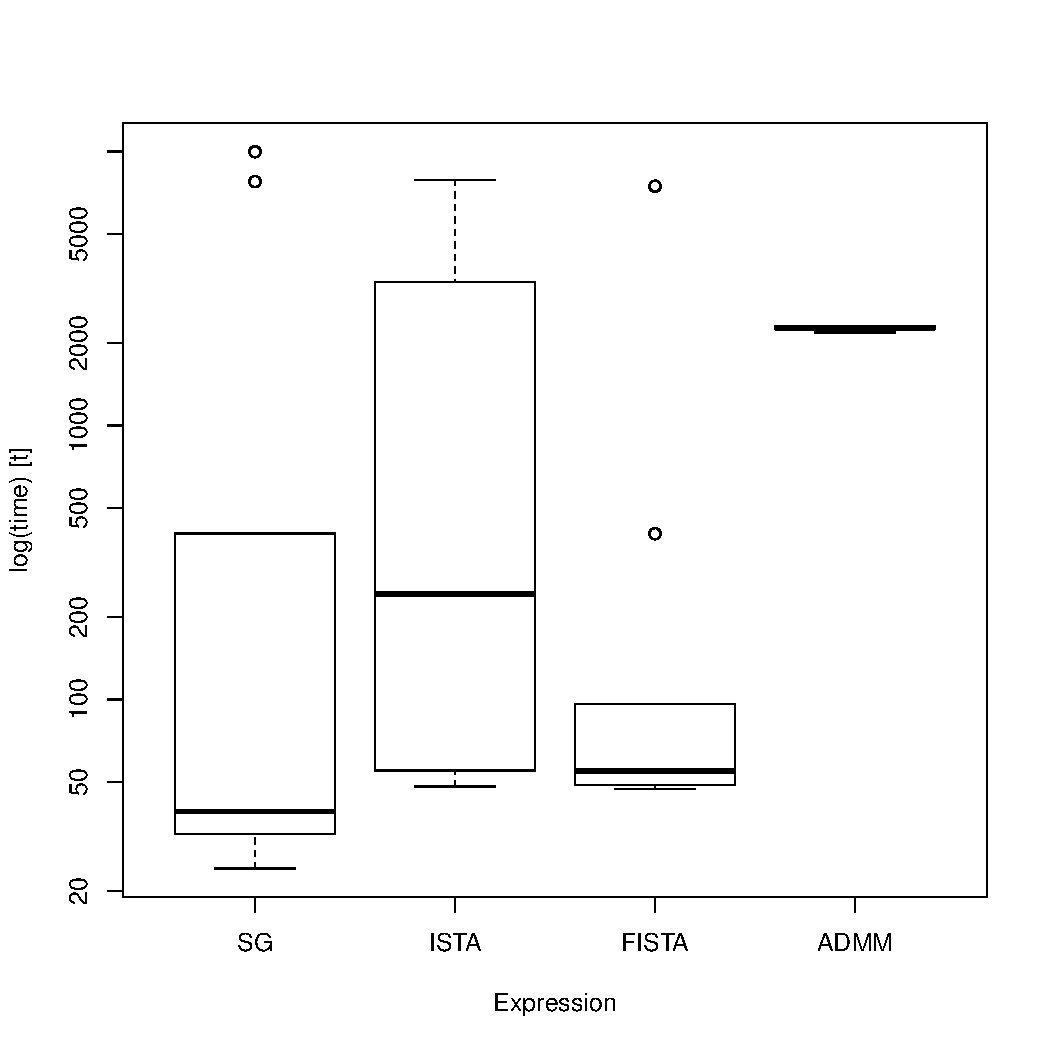
\includegraphics[width=\textwidth]{100timing-cn.pdf}
        \caption{$n=100$}
        \label{fig:100}
    \end{subfigure}
~
    \begin{subfigure}[b]{0.2\textwidth}
        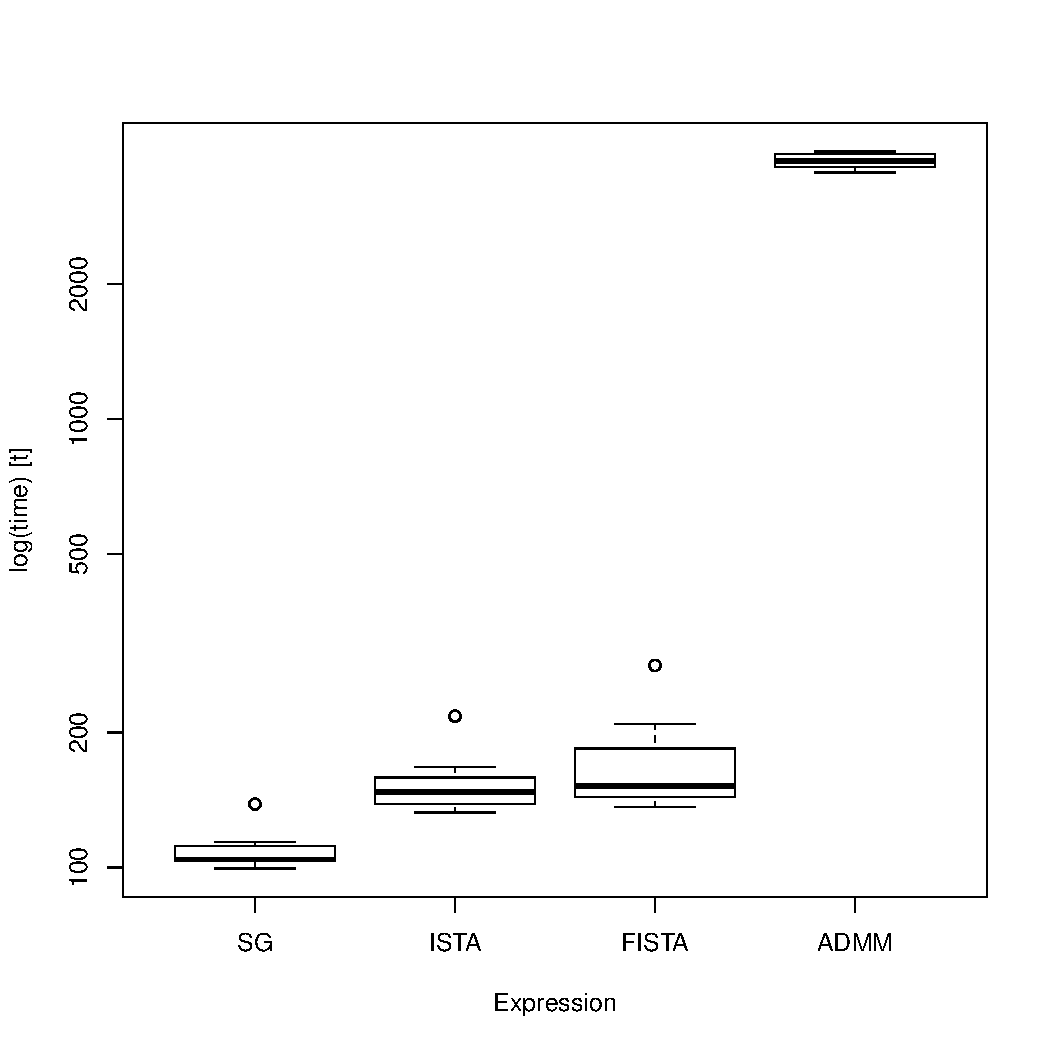
\includegraphics[width=\textwidth]{500timing-cn.pdf}
        \caption{$n=500$}
        \label{fig:500}
    \end{subfigure}
\label{fig:cvgc}
\end{figure}
\end{frame}

\begin{frame}{Relative Norm Error ($\frac{\norm{\hat{\beta}-\beta^*}_2^2}{\norm{\beta^*}_2^2}$):}
\begin{table}[ht]
\centering
\begin{tabular}{rlrrrr}
  \hline
 & Method & $n=20$ & $n=50$ & $n=100$ & $n=500$ \\ 
  \hline
1 & SG & 1.473 & $\infty$ & $\infty$ & $\infty$\\ 
  2 & ISTA& 0.015 & 0.013 & 0.0009 & 0.0011\\ 
  3 & FISTA & 0.015& 0.013 & 0.0008 & 0.0001\\ 
  4 & ADMM & 0.023 & 0.016 & 0.0025 & 0.00001\\ 
   \hline
\end{tabular}
\label{tab:relnorm}
\end{table}
\end{frame}

\begin{frame}{Data for Covariance Esimation Experiments:}
  \begin{itemize}
    \setlength{\itemsep}{10pt}
\item We set $p = 500$ and $n = 1000$.
\item Approximately $95\%$ of the entries in $\Omega^*$ were set to 0. 
\item Generate $X_i \overset{iid}{\sim} \mathcal{N}_p(0, \Omega^{-1})$ for $i = 1,...,n$. Let $X_i$ be the $i^{th}$ row of X.
 \item We compared  $\frac{\norm{\hat{\Omega}-\Omega^*}_F}{\norm{\Omega^*}_F}$ for all the methods: SG(0.463), ISTA(0.463), FISTA(0.463), ADMM(0.553). These were all inferior to glasso(0.346) discussed last week in class.
  \end{itemize}
\end{frame}

\begin{frame}
\frametitle{References}
\small
\begin{block}{}
\begin{thebibliography}{Tototo}
\bibitem{Beck} Beck, A. and Teboulle, M. (2009), {``A Fast Iterative Shrinkage-Thresholding Algorithm
for Linear Inverse Problems}, \emph{Siam J. Imaging Sciences} Vol. 2, No. 1, pp. 183-202
\bibitem{Boyd2011} Boyd, S. and Parikh, N. and Chu, E. and Peleato, B.  (2011), {``Distributed Optimization and Statistical Learning via the Alternating Direction Method of Multipliers,''} \emph{Foundations and Trends in
Machine Learning}, Vol. 3, No. 1, 1-122
\bibitem{Boyd}  Boyd, S. and Vandenberghe, L. (2009), {``Convex Optimization,''} 
\end{thebibliography}
\end{block}
\end{frame}

\end{document}
